%! TeX program = lualatex
%! TeX root = main.tex

\def\basedir{/home/theammir/labs/asd/9/res}
\input{/home/theammir/labs/asd/template/template.tex}

\usepackage{graphicx}
\usepackage[hypcap=false]{caption}

\begin{document}
\thetitlepage{9}{ІМ-42}{Туров Андрій Володимирович}{28}

\taskdesc%
\begin{enumerate}
  \item Представити у програмi напрямлений i ненапрямлений графи з заданими параметрами:
    \begin{enumerate}
      \item кількість вершин $n$;
      \item розміщення вершин;
      \item матриця суміжності $A$.
    \end{enumerate}
  \item Створити програму для формування зображення напрямленого i\\ ненапрямленого графiв у графiчному вiкнi.
\end{enumerate}

\taskspec%
$\overline{n_1 n_2 n_3 n_4} = 4228$;\\
Кількість вершин --- $10 + n_3 = 12$.\\
Розміщення вершин --- прямокутником з вершиною в центрі.

\codetext{rust}

\section{Матриці суміжності}

\begin{minipage}[t]{0.4\linewidth}
  \begin{framed}
    \noindent%
    Для напрямленого графа:\\\\
    \raggedright\footnotesize\texttt{%
      0 1 1 0 0 0 1 0 0 0 1 0\\
      0 0 0 1 0 0 0 1 0 0 1 1\\
      0 0 1 0 0 1 1 0 0 0 0 0\\
      0 0 1 1 0 1 0 1 1 1 0 1\\
      0 0 0 0 0 0 1 0 0 0 1 0\\
      0 0 0 0 0 1 0 1 0 1 0 0\\
      0 0 1 0 0 0 0 0 0 0 1 0\\
      0 0 1 0 0 0 0 0 0 1 0 0\\
      0 1 0 0 0 1 0 0 0 0 1 0\\
      1 0 1 0 0 0 0 0 0 0 0 0\\
      0 0 0 0 0 1 0 0 0 0 1 1\\
      1 0 1 1 0 1 0 0 1 1 0 1\\
    }
  \end{framed}
\end{minipage}
\hfill
\begin{minipage}[t]{0.4\linewidth}
  \begin{framed}
    \noindent%
    Для ненапрямленого графа:\\\\
    \raggedright\footnotesize\texttt{%
      0 1 1 0 0 0 1 0 0 0 1 0\\
      1 0 0 1 0 0 0 1 0 0 1 1\\
      1 0 1 0 0 1 1 0 0 0 0 0\\
      0 1 0 1 0 1 0 1 1 1 0 1\\
      0 0 0 0 0 0 1 0 0 0 1 0\\
      0 0 1 1 0 1 0 1 0 1 0 0\\
      1 0 1 0 1 0 0 0 0 0 1 0\\
      0 1 0 1 0 1 0 0 0 1 0 0\\
      0 0 0 1 0 0 0 0 0 0 1 0\\
      0 0 0 1 0 1 0 1 0 0 0 0\\
      1 1 0 0 1 0 1 0 1 0 1 1\\
      0 1 0 1 0 0 0 0 0 0 1 1\\
    }
  \end{framed}
\end{minipage}
\hfill

\pagebreak
\section{Зображення}

\begin{figure}[h!]
  \center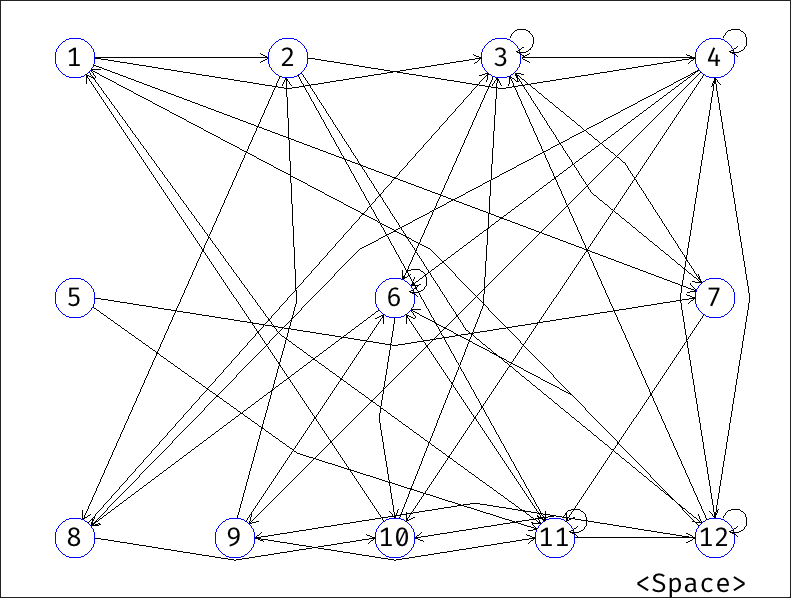
\includegraphics[width=0.5\linewidth]{directed.png}
  \caption{Напрямлений граф}
\end{figure}
\begin{figure}[ht!]
  \center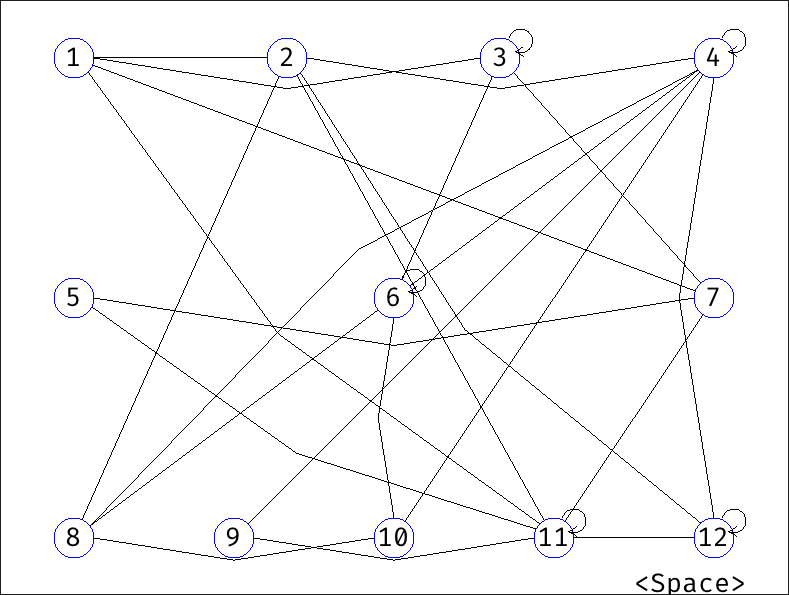
\includegraphics[width=0.5\linewidth]{undirected.png}
  \caption{Ненапрямлений граф}
\end{figure}

\conclusion%
Використав Raylib мовою програмування Rust для зображення графа за заданою матрицею суміжності.\\
За допомогою графічних примітивів намалював вершини та ребра, алгоритмічно вибираючи між прямим сполученням між колами та сполученням ламаною, що проходить (у звіті) під основним кутом $\pi/20$.\\
У програмі граф повністю представлений своєю матрицею суміжності, фактичною та відносною позицією вершин у просторі.

\end{document}

% vim: ts=2: sw=2
